\documentclass{article}
\usepackage[margin = 0.5in, top = 1in]{geometry}
\usepackage{fancyhdr}
\usepackage{physics}
\usepackage{amssymb}
\usepackage{comment}
\usepackage{verbatim}
\usepackage{graphicx}
\usepackage{hyperref}
\usepackage{amsmath}
\usepackage{float}
\usepackage{listings}
\usepackage{tikz}
\usepackage{multicol}
\pagestyle{fancy}
\hypersetup{
    colorlinks=true,
    linkcolor=blue,
    filecolor=magenta,      
    urlcolor=cyan,
    pdftitle={Overleaf Example},
    pdfpagemode=FullScreen,
}
\fancyhf{}
\setlength{\headheight}{14.49998pt}
    \graphicspath{{plots/}}

\begin{document}

\begin{titlepage}
	\centering
	
\includegraphics[width=0.6\textwidth]{EN_zwykly.png}\par
	\vspace{2cm}
	%%%% COMMENT OUT irrelevant lines among the 3 below
	{\scshape\LARGE \bfseries  Introduction to Computational Fluid Dynamics (CFD) simulations using OpenFOAM\par}
	\vfill%if you're a CS major
	%{\scshape\LARGE \& \par}                %if you're a CS & DS major
	%{\scshape\LARGE Data Science \par}      %if you're a DS major
	%\vspace{1cm}
	
	{\scshape\Large Student Team Project\par}
	%{\large \today\par}
	\vfill
	
	%%%% PROJECT TITLE
	{\huge\bfseries  Summer Semester 2023 \par}
	\vfill
	
	%%%% AUTHOR(S)
	{\Large\scshape
 Dawid Woś\\
 Joydeep Sarkar\\
  Mark Passia\\
 Mateusz Kapusta\\}
	\vspace{1.5cm}

	\vfill
	{\Large \scshape Supervised by\par
	%%%% SUPERVISOR(S)
	Rishab Prakash Sharma}


	\vfill
% Bottom of the page
\end{titlepage}
\tableofcontents

\newpage
\section{Introduction}
OpenFoam is a Computational Fluid Dynamics (CFD) framework designed for the simulations of fluids/continuum mechanics, developed initially at Imperial Collage London. Since the creation 
software have been popularized as a open and easy to extend framework suitable for different type of simulations ranging from simple diffusion up to multiphase fluids and Magnetohydrodynamics 
(MHD). It is written in C++ language and utilizing modern features like objective oriented programing (OOP). 

In this project a basic introduction to the CFD using OpenFoam was given. Report is structured as follows. In the first part practical introduction to OpenFoam 
will be given including mesh generation, solver creation and practical considoration will be given. In second part some interesting cases will be considered together with analitical 
comparison.

\section{OpenFoam programing}
In order to provide an easy introduction for OpenFoam a simple diffusion case will be considered in this chapter.
At the end of this chapter reader should be able to reproduce this simple example from the beginning.
We would like to solve a diffusion equation
\begin{equation}
    D_T\laplacian{U} + \pdv{T}{t} = 0,
\end{equation} on the block with two different temperatures at both sides.

Before diving into the specifics of each simulation step, let's take a brief overview of typical OpenFOAM case directory,
which is structured into several folders and files. For a simple heat diffusion case, the directory looks as follows: 

 \begin{lstlisting}
heatDiffusionCase/
|-- 0/
    |-- T
|-- constant/
    |-- transportProperties
|-- system/
    |-- controlDict
    |-- fvSchemes
    |-- fvSolution
\end{lstlisting}

\noindent The files are grouped such that each folder contains files associated with a specific tasks:

\begin{itemize}
    \item \textbf{0/T}: This file contains the initial and boundary conditions for the temperature field.
    \item \textbf{constant/thermophysicalProperties}: This file defines the physical properties of the materials involved in the simulation.
    \item \textbf{system/controlDict}: This file controls the overall execution of the simulation, including start and stop times and the write interval.
    \item \textbf{system/fvSchemes}: This file specifies the numerical schemes used for different terms in the equations.
    \item \textbf{system/fvSolution}: This file defines the solvers and related settings for the simulation.
\end{itemize}


\subsection{Mesh generation}
In OpenFOAM, the geometry of the domain is defined using mesh files. For a simple heat diffusion simulation, we create the mesh using the \texttt{blockMesh} utility,
which reads the mesh description from a file named \texttt{blockMeshDict} located in the \texttt{system} directory.
In which both the geometry and the mesh of the simulated object are defined.
Here are the keywords used in the exaple blockMeshDict file\footnote{It is also possible to simulate in OpenFOAM using third-party CAD models.
This can be done by converting the CAD models into a suitable mesh format using tools like \texttt{snappyHexMesh} or third-party software such as \texttt{gmsh}.}:


\begin{itemize}
    \item \textbf{FoamFile \{ ... \}}: This section defines metadata for the file, including version, format, and object type, which at this point is the blockMeshDict.
    \item \textbf{scale 1;}: Sets the scale factor for the geometry.
    \item \textbf{xmin}, \textbf{xmax}, \textbf{ymin}, \textbf{ymax}, \textbf{zmin}, \textbf{zmax}: Define the dimensions for the block.
    \item \textbf{xcells}, \textbf{ycells}, \textbf{zcells}: Define the number of cells in the x, y, and z directions, respectively.
    \item \textbf{vertices \{ ... \}}: Defines the vertices of the blocks. Each vertex is given by `(x y z)`.
    \item \textbf{blocks \{ ... \}}: Defines the hexahedral blocks using the vertices specified. Each block is assigned the number of cells and grading.
    \begin{itemize}
        \item \textbf{simpleGrading (1 1 1)} specifies the mesh grading in the x, y, and z directions. Grading controls the distribution of cells within the block.
        Values of 1 means no expansion or contraction, resulting in uniformly sized cells.
    \end{itemize}
    \item \textbf{boundary \{ ... \}}: Defines the boundary patches and their types, such as `wall`. Each boundary is associated with specific faces of the blocks.
\end{itemize}

\noindent The example file used, which can be viewed in the appendix, results in the following geometry and mesh, which will subsequently be simulated; see Fig. \ref{fig:UsedMesh}.

\begin{figure} [H]
    \centering
    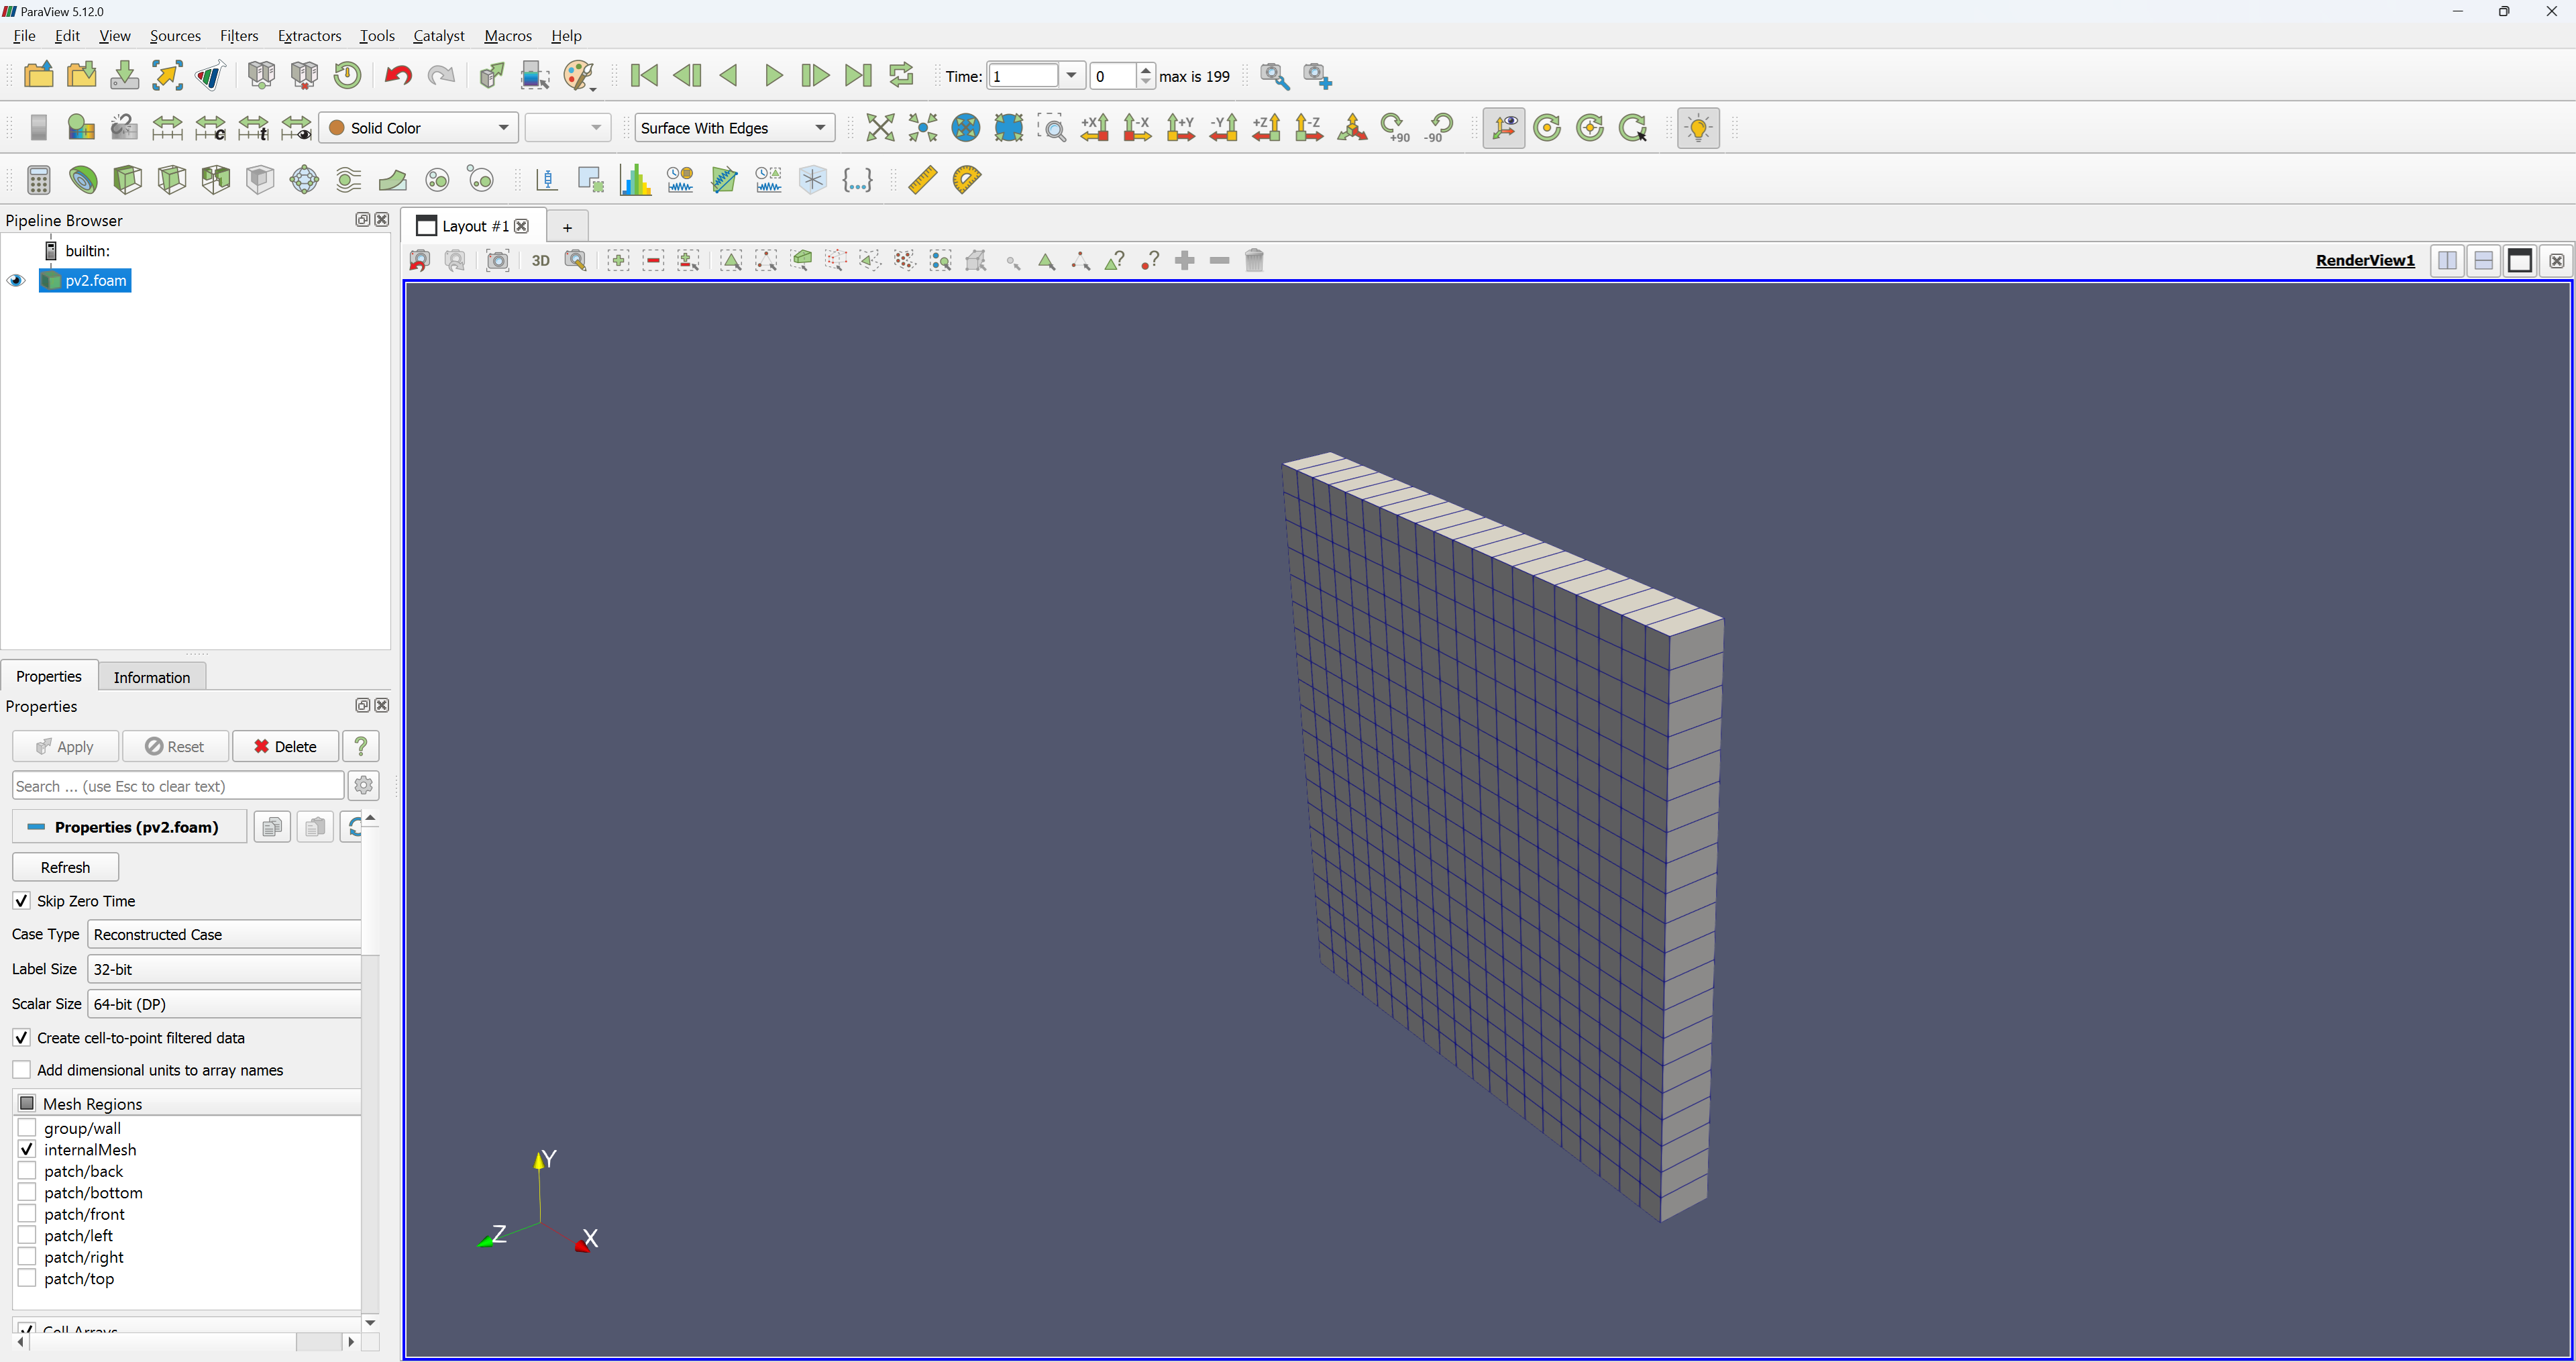
\includegraphics[width= 15cm]{Example_geometry.png}
    \caption{Created geometry and mesh shown in Paraview.}
    \label{fig:UsedMesh}
\end{figure}

\subsection{Material properties}
Every simulation of a physical object requires inputting the material properties of the simulated object, be it a fluid or a solid. In OpenFOAM the material properties for the simulation are defined in the \texttt{constant/transportProperties} file. In our case the only variable which can be changed in that file is thermal diffusivity, abbreviated as \texttt{DT}. It is a measure of how quickly temperature changes occur within a material when it is subjected to a thermal gradient. The corresponding file structure is as follows:

\begin{verbatim}
FoamFile
{
    version     2.0;
    format      ascii;
    class       dictionary;
    location    "constant";
    object      transportProperties;
}

DT              0.01;
\end{verbatim}




\subsection{Boundary and initial conditions}
In order to define the starting values and the boundary conditions for the simulated setup, we need to manipulate the content of the \texttt{0/T} file. Next, let's take a look at each command of the following example file and inspect what it achieves.

\begin{verbatim}
FoamFile
{
    version     2.0;
    format      ascii;
    class       volScalarField;
    object      T;
}

dimensions      [0 0 0 1 0 0 0];
internalField   uniform 273;
boundaryField
{
    top{
        type            fixedValue;
        value           uniform 573;
    }

    bottom{
        type            fixedValue;
        value           uniform 273;
    }

    left{
        type            zeroGradient;
    }
    (...)
}
\end{verbatim}


\begin{itemize}
    \item \textbf{dimensions}: This line defines the physical dimensions of the field variable. The vector \([0 \ 0 \ 0 \ 1 \ 0 \ 0 \ 0]\) indicates that the variable has the dimensions of temperature.
    \begin{itemize}
        \item The dimensions in the \texttt{dimensions} entry of the OpenFOAM file are specified in the following order $[M \ L \ T \ \Theta \ N \ I \ J]$, where:
        \begin{itemize}
            \item \(M\) is mass
            \item \(L\) is length
            \item \(T\) is time
            \item \(\Theta\) is temperature
            \item \(N\) is quantity of substance
            \item \(I\) is electric current
            \item \(J\) is luminous intensity
        \end{itemize}
    \end{itemize}

    \item \textbf{internalField}: This defines the initial condition for the entire domain.
    \begin{itemize}
        \item \textbf{uniform 273}: Sets the initial temperature to a uniform value of 273 Kelvin throughout the domain.
    \end{itemize}

    \item \textbf{boundaryField}: This section specifies the boundary conditions for the field variable at the boundaries of the domain.
    \begin{itemize}
        \item \textbf{top}:
        \begin{itemize}
            \item \textbf{type fixedValue}: Specifies that the boundary condition is a fixed value.
            \item \textbf{value uniform 573}: Sets the temperature at the top boundary to a uniform value of 573 Kelvin.
        \end{itemize}

        \item \textbf{bottom}:
        \begin{itemize}
            \item \textbf{type fixedValue}: Specifies that the boundary condition is a fixed value.
            \item \textbf{value uniform 273}: Sets the temperature at the bottom boundary to a uniform value of 273 Kelvin.
        \end{itemize}

        \item \textbf{left, right, front, back}:
        \begin{itemize}
            \item \textbf{type zeroGradient}: Specifies a zero gradient boundary condition, 
                meaning there is no change in temperature across these boundaries. This effectively makes these boundaries insulating or adiabatic, preventing heat flux through them.
        \end{itemize}
    \end{itemize}
\end{itemize}

\subsection{Numerical Schemes}
After determination of the grid and equation, we need to translate differential equation to our grid. There are may different types of 
challanges associated with the choice of numerical schemes. All properties associated with schemes are defined in \texttt{system/fvSchemes} file.
A simple example of such directory may look like this:

\begin{verbatim}
FoamFile
{
    version     2.0;
    format      ascii;
    class       dictionary;
    location    "system";
    object      fvSchemes;
}
// * * * * * * * * * * * * * * * * * * * * * * * * * * * * * * * * * * * * * //

ddtSchemes
{
    default         Euler;
}

gradSchemes
{
    default         Gauss linear;
}

laplacianSchemes
{
    default         Gauss linear orthogonal;
    laplacian(DT,T) Gauss linear corrected;
}

interpolationSchemes
{
    default linear;
}

\end{verbatim}
Let's start with \texttt{ddTSchemes}. This entry specifies how a time derivative is translated. In case of simple Euler scheme we are approximating
\begin{equation}
    \pdv{X}{t} \approx \frac{X_{i+1}-X_{i}}{\Delta t},
\end{equation} where $\Delta t$ is a timestep of our simulation. There are few other schemes that might be used such as a  Crank-Nicolson time scheme.
In similar manner other entries control how other part of equation are handled. Let's take a closer look at \texttt{gradSchemes}.
A Gauss keyword states, that a Gauss theorem is used to compute 
\begin{equation}
    \grad{U} = \frac{1}{V} \sum_f \vb{S_f} U_f,
\end{equation} where $V$ stands for the volume of the cell, $\vb{S_f}$ stands for the normal vector 
to the face $f$ and $U_f$ is a {\it approximate} value of field $U$ at face $f$. This is where the second keyword comes in, as 
\texttt{linear} specifies how $U_f$ is beeing calculated. In this case we are using linear approximation and assuming mean value of 
$U$ field in two neighbouring cells separated by face $f$. There are different schemes that can be used here, some can be field-dependent as a \texttt{upwind} scheme 
or can be adjusted with additional parameters like \texttt{LimitedLinear}.


\subsection{Writing solvers}
\subsubsection{Diffusion}
All of previous chapters explained how to write a geometry for a OpenFoam case and how to to use numerical schemes. In this chapter 
an introduction will be given on the solver creation. Before we dive into the details we need to take a moment to understand how fields work. 
Usually field are defined in the {\it center} of the cell (as for example temperature in diffusion case). Hence, we start our solver with 
\begin{verbatim}
volScalarField T
(
    IOobject
    (
        "T",
        runTime.timeName(),
        mesh,
        IOobject::MUST_READ,
        IOobject::AUTO_WRITE
    ),
    mesh
);
\end{verbatim}
We have specified an object with type \texttt{volScalarField} that we need to read at the beginning (from file \texttt{0/T}) and which will be automatically saved.
We are also specifing mesh on which our field is anchored.
Than we have a simple loop 
\begin{verbatim}

while (simple.loop())
    {
        Info<< "Time = " << runTime.timeName() << nl << endl;

        while (simple.correctNonOrthogonal())
        {

            fvScalarMatrix TEqn
            (
                fvm::ddt(T)
               -fvm::laplacian(DT, T)
             ==
                fvOptions(T)
            );
            fvOptions.constrain(TEqn);
            TEqn.solve();
            fvOptions.correct(T);
        }
        #include "write.H"
        runTime.printExecutionTime(Info);
}
\end{verbatim}
We are defining an equation with type \texttt{fvScalarMatrix} which is defined with operators \texttt{fvm::ddt} and \texttt{fvm::laplacian(DT,T)}.
Both of those are translated to the discretized matrix equation using numerical schemes that we have already covered. There are also more 
advanced options present as constrains and corrections which we won't delve into. Usually this is enough for such solvers to work in most basic 
possible setup.

\subsubsection{Transport equation}
Now let's start with basic modification to the diffusion equation known as the transport equation:
\begin{equation*}
    \pdv{T}{t} - D \laplacian{T} + \div{(T\vb{u})} = 0,
\end{equation*}
where $\vb{u}$ denotes the velocity of the fluid. In general velocity needs to be obtained with the help of the 
continuity equation and Euler equation. Here, as a simplification we are treating it as a know field (constant with time).

While diffusion equation is parabolic in nature, after including transport element it becomes hyperbolic in nature. In order to solve the problem, one defines \textbf{fluxes},
which are denoted as $\phi$. In the discretization scheme we are once again defining cells, with centers and surfaces.
While $\vb{u}$ is a vector field defined in the \textbf{center}
of the cells, $\phi$ is defined as the $\phi_i = u_i S_i$, where $u_i$ is a interpolated value of i-th component of the velocity, $S_i$ is a surface of the cell.
Basic idea involves using the values defined at surface instead of those defined at centers to evaluate the derivative $\pdv{x}$, which makes the scheme more robust.
While $\vb{u}$ has $3$ components, $\phi$ has $8$ defined at each of centers of the cell's surfaces. In OpenFoam there is clear distinction between the objects:

\begin{verbatim}
    volVectorField U
    (
    IOobject
    (
        "U",
        runTime.timeName(),
        mesh,
        IOobject::MUST_READ,
        IOobject::AUTO_WRITE
    ),
    mesh
    );
    surfaceScalarField phi
    (
    IOobject
    (
        "phi",
        runTime.timeName(),
        mesh,
        IOobject::NO_READ,
        IOobject::NO_WRITE
    ),
    fvc::flux(U)
    );
\end{verbatim}
Velocity field is defined as \texttt{volVectorField} while $\phi$ is \texttt{surfaceScalarField}.
In the declaration of $\phi$ we demand not to write down the field and do not read it. Whole field is defined using \texttt{flux} method which 
tells OpenFoam to automatically tie the definition with $\vb{u}$.
We also need to modify the equations in the main solver body.
\begin{verbatim}
    phi = fvc::flux(U);
    fvScalarMatrix TEqn
    (
        fvm::ddt(T) 
        +fvm::div(phi,T)
        -fvm::laplacian(DT, T)
        ==
        fvOptions(T)
    );
\end{verbatim}
Two of those options combined are enough to create a new solver for the OpenFoam.
We also need to add additional term in the \texttt{system/fcSchemes} file as we need a scheme for a divergence.
\begin{verbatim}
    divSchemes
    {
        default none;
        div(phi,T) Gauss <keyword>
    }
\end{verbatim}
where \texttt{<keyword>} is a name of the method we would like to use for divergence computation.
Simillar keywords are available as with the gradient as divergence calculation can be essentially reduced to the gradient computation. 

\section{OpenFoam simulations}
This whole section will contain various tests and cases, some with analitical solutions. 
\subsection{Diffusion equation + Transport}
\begin{figure}
    \begin{center}
        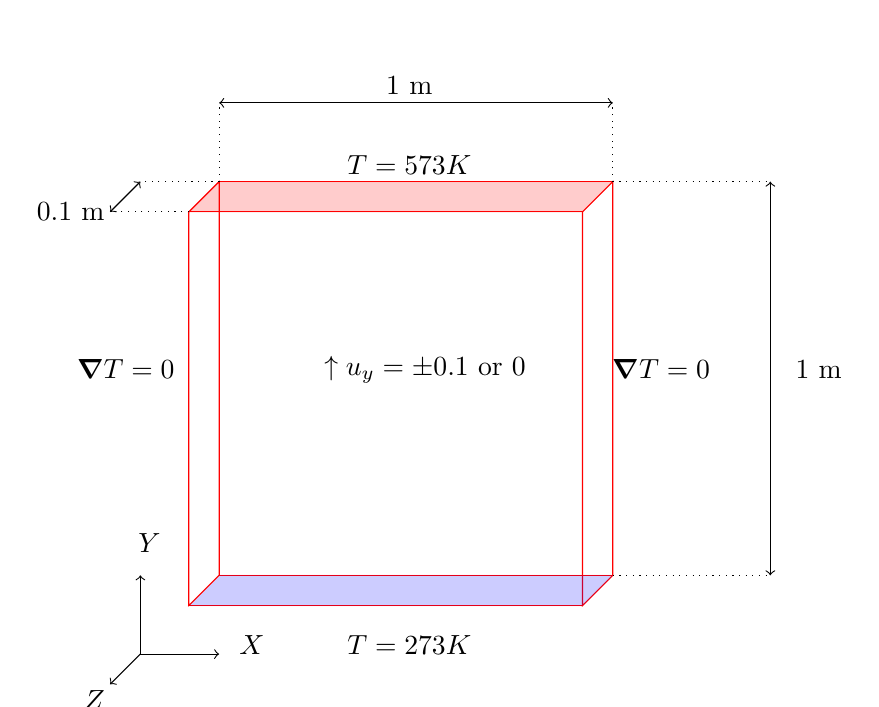
\begin{tikzpicture}
        \pgfmathsetmacro{\cubex}{5}
        \pgfmathsetmacro{\cubey}{5}
        \pgfmathsetmacro{\cubez}{1}
        \draw[red] (0,0,0) -- ++(-\cubex,0,0) -- ++(0,-\cubey,0) -- ++(\cubex,0,0) -- cycle;
        \draw[red] (0,0,-\cubez) -- ++(-\cubex,0,0) -- ++(0,-\cubey,0) -- ++(\cubex,0,0) -- cycle;
        \draw[red] (0,0,0) -- ++(0,0,-\cubez) -- ++(0,-\cubey,0) -- ++(0,0,\cubez) -- cycle;
        \draw[red,fill = blue,opacity=0.2] (0,-\cubey,0) -- ++(-\cubex,0,0) -- ++(0,-0,-\cubez) -- ++(\cubex,0,0) --cycle;
        \draw[red] (-\cubex,0,0) -- ++(0,0,-\cubez) -- ++(0,-\cubey,0) -- ++(0,0,\cubez) -- cycle;
        \draw[red,fill=red,opacity=0.2] (0,0,0) -- ++(-\cubex,0,0) -- ++(0,0,-\cubez) -- ++(\cubex,0,0) -- cycle;
        \draw[line width=5pt] (-2.2,0.6) node {$T = 573 K$};
        \draw[line width=5pt] (-2.2,-5.5) node {$T = 273 K$};
        \draw[line width=5pt] (1,-2) node {$\grad T = 0$};
        \draw[line width=5pt] (-5.8,-2) node {$\grad T = 0$};
        \draw[line width=5pt] (-2,-2) node {$ \uparrow u_y = \pm 0.1 \textrm{ or  } 0$};
        \draw[->] (-6,-6,-1) -- ++(1,0,0);
        \draw[->] (-6,-6,-1) -- ++(0,1,0);
        \draw[->] (-6,-6,-1) -- ++(0,0,1);
        \draw[line width=5pt] (-5.5,-4.2,0) node {$Y$};
        \draw[line width=5pt] (-4.2,-5.5,0) node {$X$};
        \draw[line width=5pt] (-6.2,-6.2,0) node {$Z$};
    
        \draw[dotted] (0,0,-\cubez) -- (0,1,-\cubez);
        \draw[dotted] (-\cubex,0,-\cubez) -- (-\cubex,1,-\cubez);
        \draw[<->] (0,1,-\cubez) -- (-\cubex,1,-\cubez);
        \draw[line width=5pt] (-2.2,1.6) node {$1$ m};
    
        \draw[dotted] (-\cubex,0,-\cubez) -- (-\cubex-1,0,-\cubez);
        \draw[dotted] (-\cubex,0,0) -- (-\cubex-1,0,0);
        \draw[<->] (-\cubex-1,0,0) -- (-\cubex-1,0,-\cubez);
        \draw[line width=5pt] (-6.5,0) node {$0.1$ m};
    
        \draw[dotted] (0,0,-\cubez) -- ++(2,0,0);
        \draw[dotted] (0,-\cubey,-\cubez) -- ++(2,0,0);
        \draw[<->] (2,0,-\cubez) -- (2,-\cubey,-\cubez);
        \draw[line width=5pt] (3,-2) node {$1$ m};
    
    \end{tikzpicture}
    \end{center}
    \caption{Diagram of the block used in the simulations}\label{fig:block}
\end{figure}
Let's start with geometry of block presented in Figure \ref{fig:block}. Upper side of the block is kept at $573$ K while lower part is kept at 
$273$ K. We also include "wind" in the $Y$ direction that will slightly modify our solution. 
We assume, that the wind is uniform in whole block.
Without the wind one expects steady state that 
\begin{equation}
    \laplacian{T} = 0,
\end{equation}
which in our case gives us linear rise from lower to upper value of temperature. This image slightly changes 
if we include wind.
We have than 
\begin{equation}
    \pdv[2]{T}{y} + \frac{u_y}{D_T}\pdv{T}{y} = 0.
\end{equation}
This solution has slightly different form with exponential rise/fall, with characteristic length  $\lambda  = \frac{D_T}{u_y}$.

Three separate cases are considered in total: no wind case and two cases with moderate velocity up and down the hill.
In our simulations we assumed $D_T  = 0.01$ and $u_y = \pm 0.1$ in wind cases. 
In order to simulate cases PBiCGStab solver with DILU preconditioner were used. All numerical schemes used simple linear interpolations together with 
Euler time scheme. Comparison between numerical and analitical solutions is presented in Figure \ref{fig:com}. 
Paraview visulization of upwind case is presented in Figure \ref{fig:3d}. In case of zero velocity we are recovering simple linear form. In case of positive value of flow we are getting very steep 
temperature profile as the velocity "blocks" flow of the temperature. On the other hand if velocity is in other direction velocity is "spreading" temperature.
In all cases we are getting around $0.5$ K error despite only using $N = 51$ cells in $Y$ direction.
\begin{figure}[!tbp]
    \centering
    \begin{minipage}[b]{0.45\textwidth}
        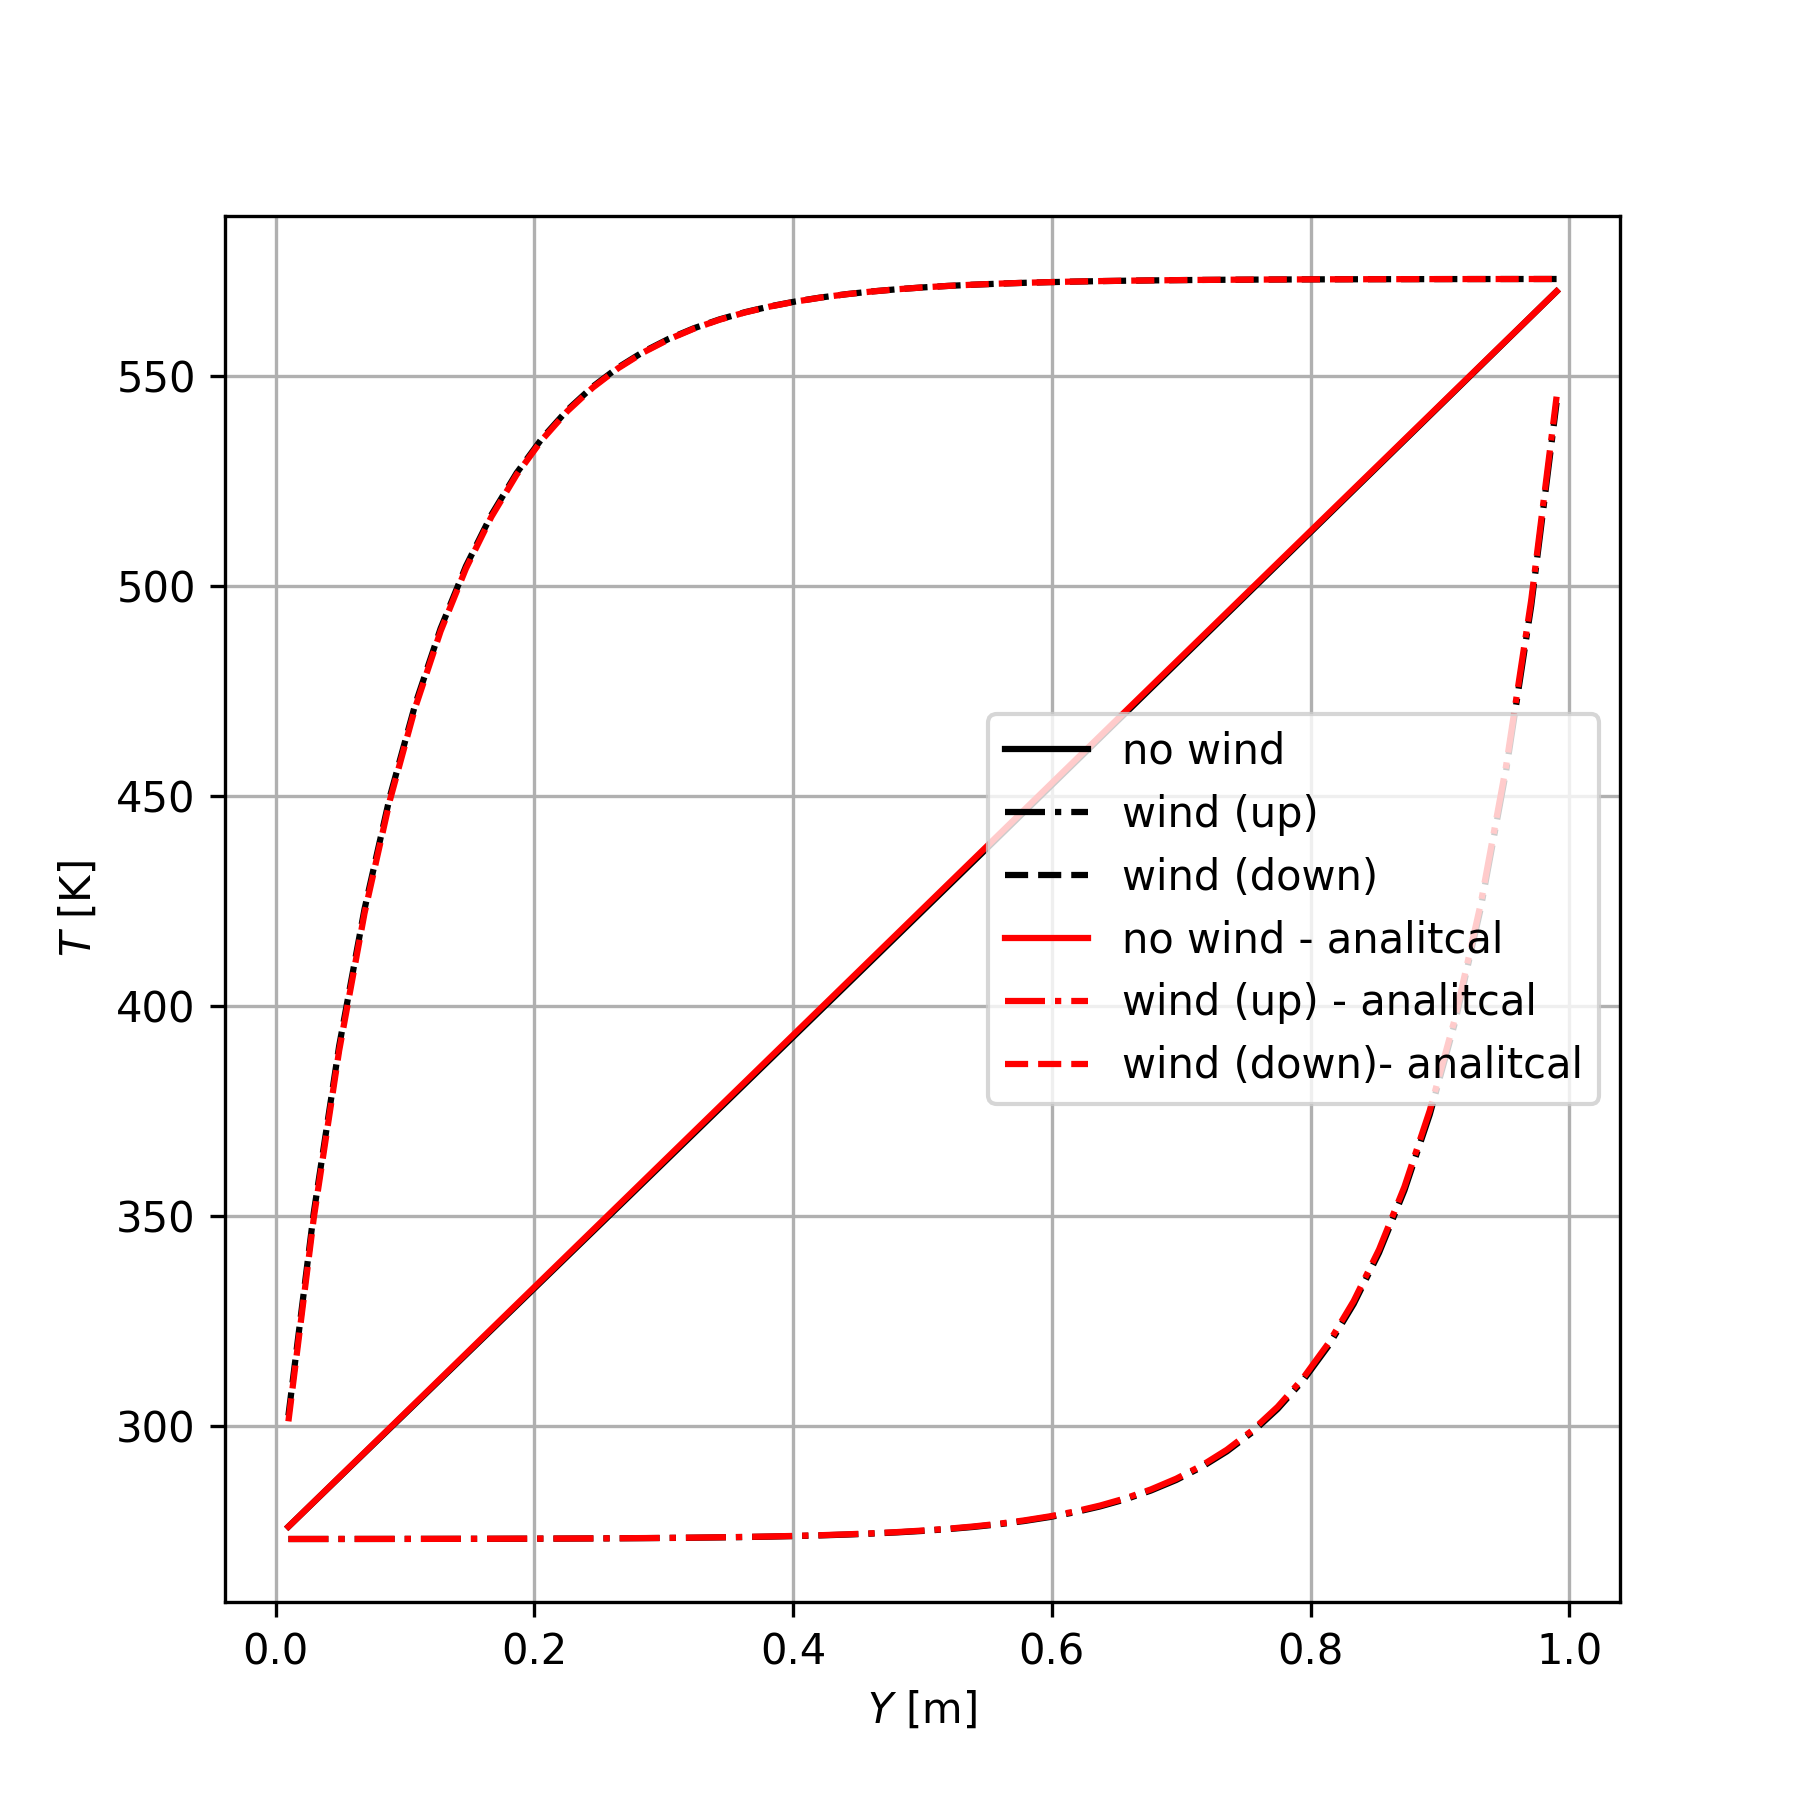
\includegraphics[width = \textwidth]{comp.png}
        \caption{Comparison of velocity profile with and without velocity field (up stands for the positive $u_y$).}\label{fig:com}
    \end{minipage}
    \hfill
    \begin{minipage}[b]{0.45\textwidth}
        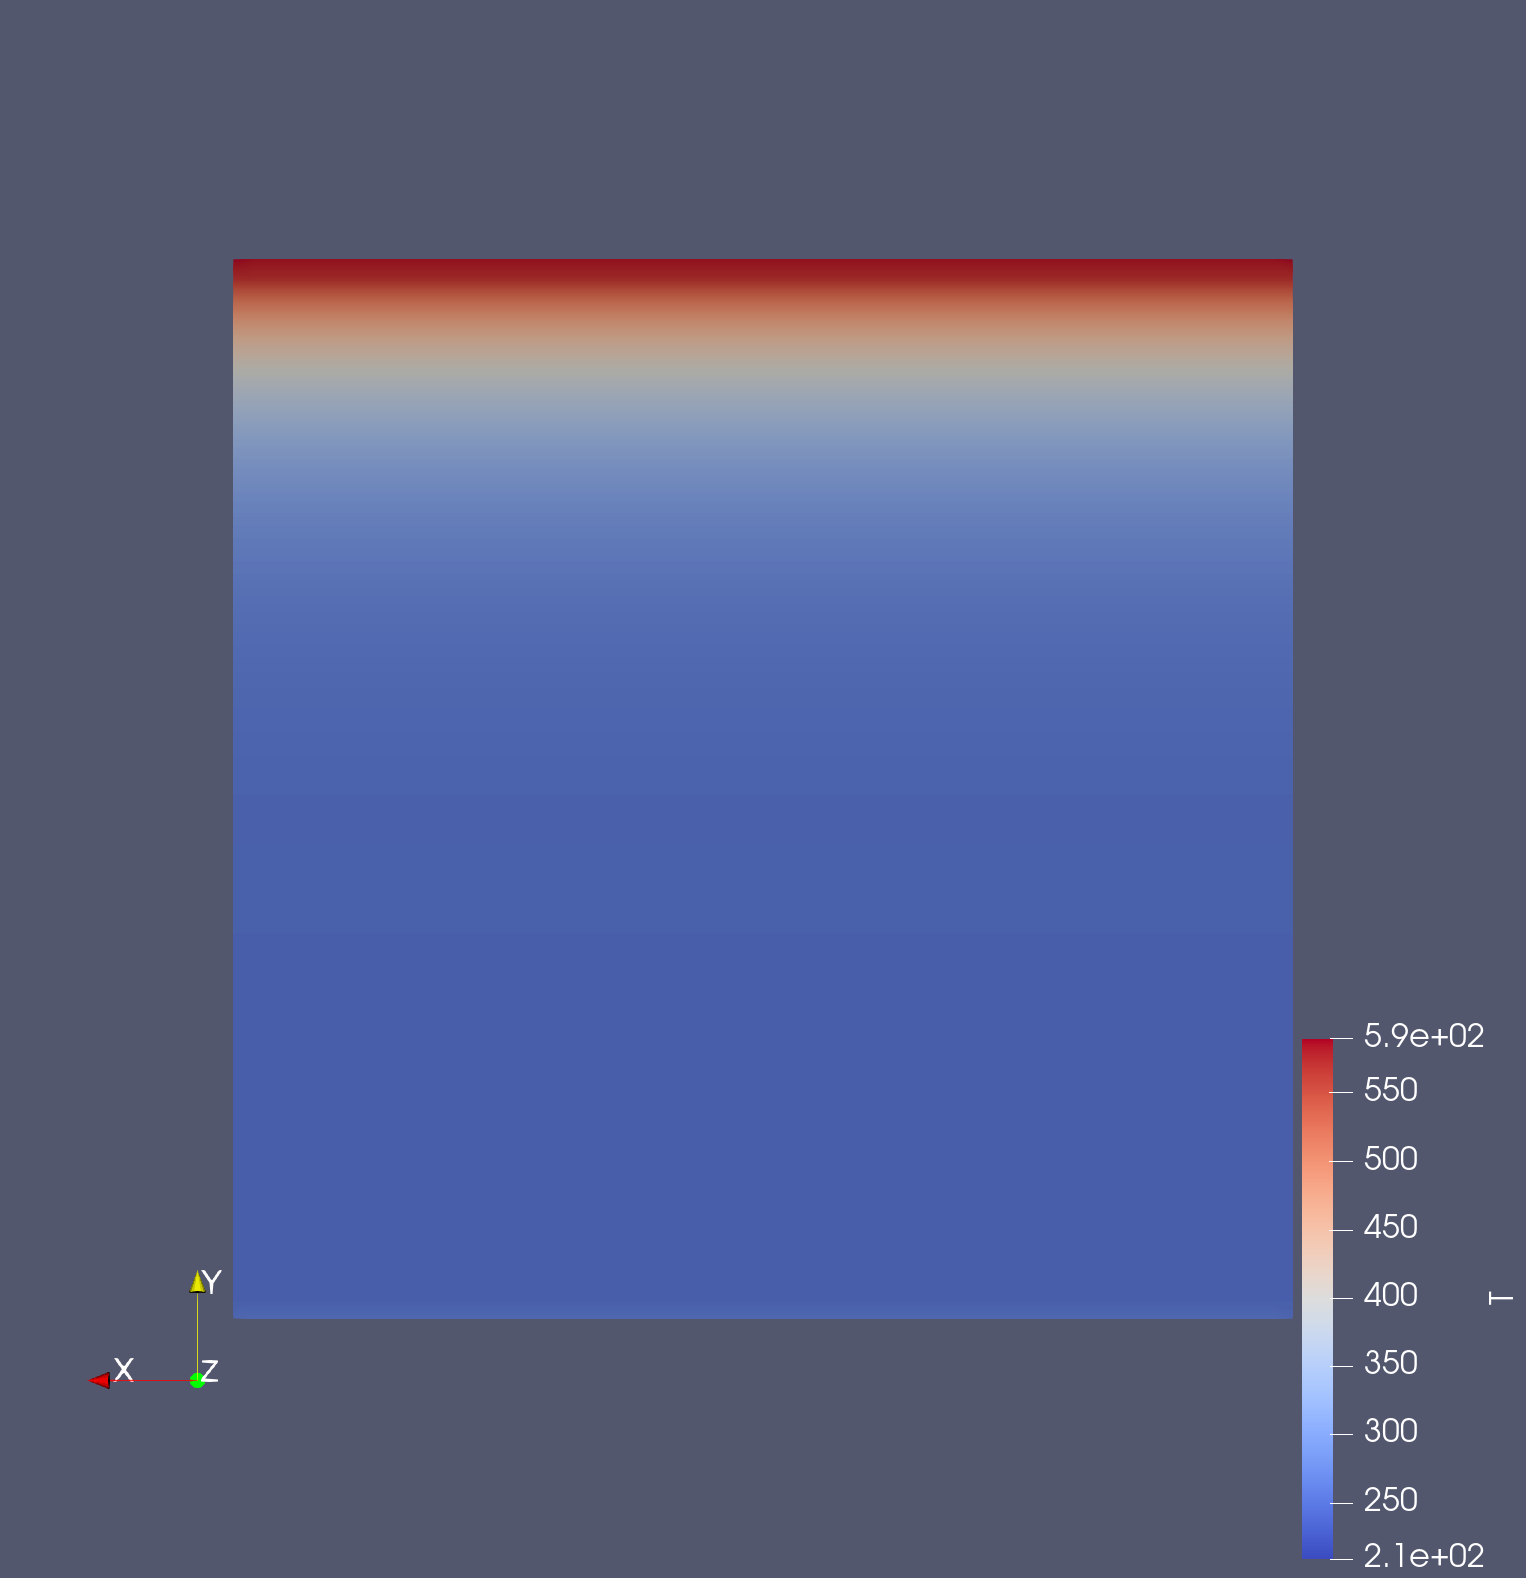
\includegraphics[width = \textwidth]{mod_3d.png}
        \caption{Temperature profile in the $Y$ direction after reaching steady state with nonzero upflow velocity.}\label{fig:3d}
    \end{minipage}
\end{figure}

\subsection{Couette flow}
Now let's move to the Coutte flow in pipe. Here, a viscous laminar flow will be considered with incompressible solver called \texttt{icoFoam}.
There are two variables $\vb{u}$ and $p$ and two equations
\begin{align}
    \div{\vb{u}} = 0,\\
    \pdv{\vb{u}}{t} + (\vb{u}\cdot \grad)\vb{u} = \nu \laplacian{\vb{u}} -\grad{p}.\\
\end{align}
Here, pressure $p$ represents in fact pressure divided by the density (pressure density). Incompressible flow is a good approximation as long as considered velocities are smaller than local speed of 
sound, which is important to keep in mind. We are considering flow in pipe, which is purely in $Z$ direction. Moreover, we are assuming flow is symmetrical and hence depends only on 
$r$ variable. It's possible to prove in such case, that velocity profile inside pip should be parabolic.
Here is where the things get a little bit tricky. Usually in such cases we are assuming, that we have translational symmetry. This usually can be realized in case of very long system.
Here, we can employ a different approach. OpenFoam provides us with a \textbf{cyclic} boundary condition. Those allow for realizing various for of translational boundaries.
First we need to start with \texttt{blockMeshDict}.
\begin{verbatim}
    boundary
    (
        inlet
        {
            type  cyclic;
            neighbourPatch outlet; 
            faces
            (
                <faces>
            );
        }
        outlet
        {
            type  cyclic;
            neighbourPatch inlet; 
            faces
            (
                <faces>
            );
        }
    <pipe>
    )        
\end{verbatim}
We are writing down a different type of boundary called \texttt{cyclic}. We also need to specify boundary condition in our fields, here in case of velocity 
$\vb{u}$
\begin{verbatim}
boundaryField
{
    pipe
    {
        type noSlip;
    }
    inlet
    {
        type cyclic;
        neighbourPatch outlet;
        transform translational;
    }
    outlet
    {
        type cyclic;
        neighbourPatch inlet;
        transform translational;
    }
}
\end{verbatim}
This guaranties that our case will have translational symmetry and hence we do not need a long pipe. 

\texttt{icoFoam} solvers is a little bit more elaborate than laplacian solver and detailed description of it is beyond the scope of the report.
As it is one of most popular solvers available, we won't delve into the details of \texttt{fvSchemes} and \texttt{fcSolution} files.
Unfortunately fluid simulations are quite slow compared to the simple laplacian solver so simulations were accelerated using OpenFoam MPI interface. 
In simulations viscosity $\nu = 0.01$ was used with initial uniform velocity profile, with velocity $u_z = 0.1$ m/s. After $400$ s 
final velocity profile was plotted and is presented with Paraview block rendering in Figure \ref{fig:pipe_block} and Figure \ref{fig:pipe_profile}.
As one can clearly see velocity profile is parabolic as one expects from the theoretical point of view.
\begin{figure}[!tbp]
    \centering
    \begin{minipage}[b]{0.45\textwidth}
      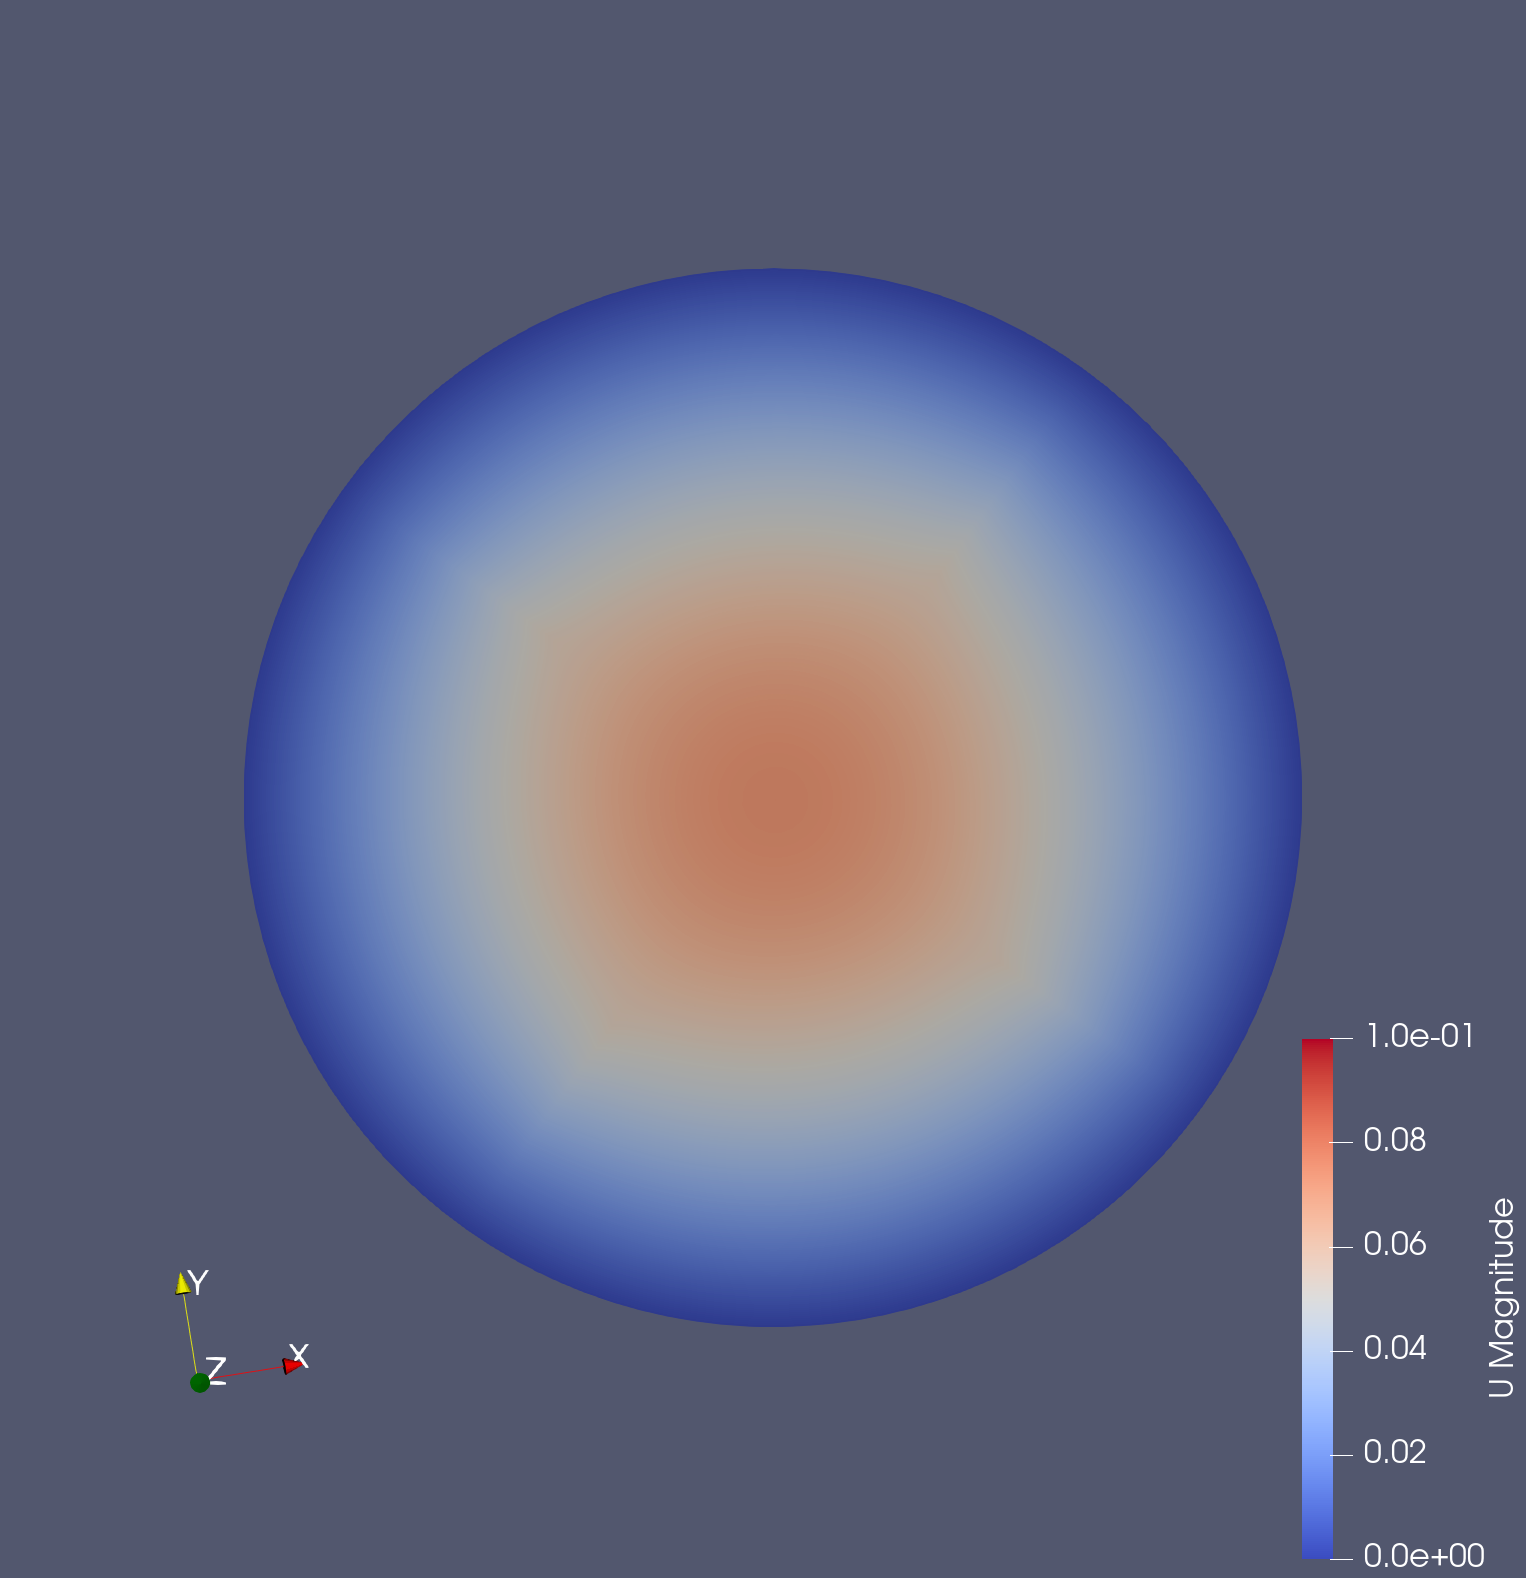
\includegraphics[width=\textwidth]{block.png}
      \caption{Paraview rendering of velocity in block.}
      \label{fig:pipe_block}
    \end{minipage}
    \hfill
    \begin{minipage}[b]{0.45\textwidth}
      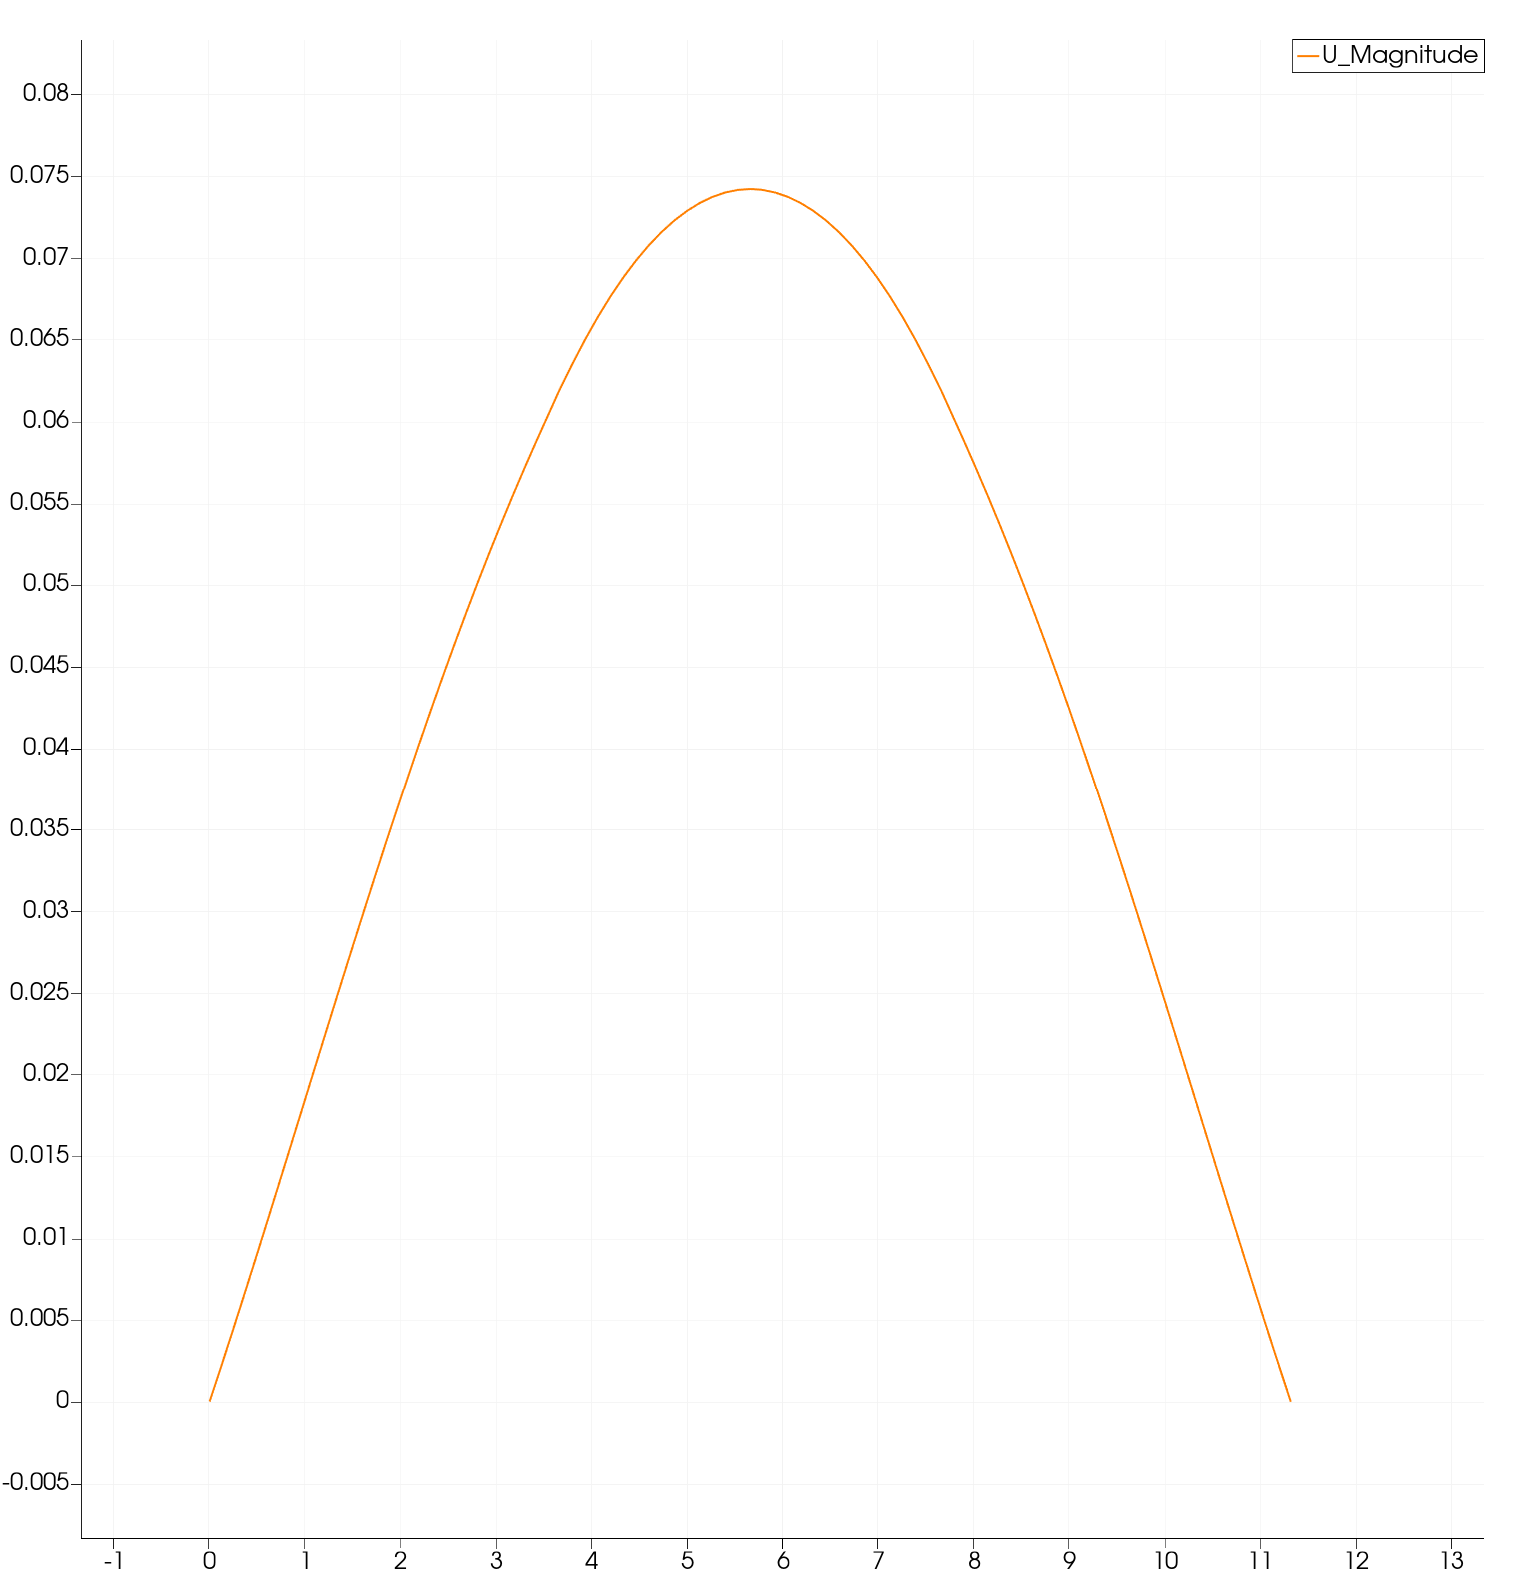
\includegraphics[width=\textwidth]{profile.png}
      \caption{Velocity profile inside the pipe.}
      \label{fig:pipe_profile}
    \end{minipage}
  \end{figure}
\end{document}

